\def\red#1{\textbf{\color{javared}#1}}
\def\blue#1{\textbf{\color{javadocblue}#1}}

\begin{center}
	\Huge \textbf{Собственно, матстат...}
\end{center}
\section{Описова статистика.}
\subsection{Основнi поняття математичної статистики.}
 \begin{itemize}
 \item\textbf{\color{javared} Математична статистика} - це розділ математики, в якому вивчаються методи збору, систематизації та обробки інформації з метою виявлення існуючих закономірностей.
   \end{itemize}
     У математичній статистиці набір даних розглядається як реализація або спостереження деякої випадкової величини (в.в.) $\xi$, яка визначена на деякому ймовірнісному просторі $\left( \Sigma, F, P \right)$, пов'язаний із стохастичним експериментом.
   \begin{itemize}
     \item \textbf{\color{javared} Генеральна сукупність} (population) -  це (як правило, невідомий) ймовірнісний розподіл $F$ в.в. $\xi$, що спостерігається (ймовірнісна міра $P$)
     \item \textbf{\color{javared} Вибірка} (sample) - це набір незалежних в.в. $\xi_1, \xi_2 ,..., \xi_n$, кожна з яких має розподіл $F$. При цьому $n$ називається об'ємом вибірки.
     \item \textbf{\color{javared} Реалізація вибірки} - це значення $x_1 , x_2 , ... , x_n$ або $\overrightarrow{x} = \begin{bmatrix}
      x_1 & \cdots & x_n
     \end{bmatrix}$, які прийняли в.в. $\xi_1 , ... , \xi_n$ в результаті конкретного стохастичного експерименту. При цьому $x_k$ називається \textbf{\color{javadocblue} варiантою}. Тобто:
     $$
     \begin{gathered}
      \left( \Sigma , F, P \right)\\
      \omega_o \in \Sigma
     \end{gathered} \qquad x_1 = \xi_1(\omega_0)\ , \ \cdots \ , \  x_n  = \xi_n (\omega_0) \qquad \begin{array}{r}
      \text{Вибірка: } (\xi_1 , ..., \xi_n) \\
      \text{Реал. вибірки: } (x_1 , ... , x_n)
     \end{array}
     $$
 \end{itemize}
Основою будь-яких висновкiв щодо властивостей г.с. $F$ є \textbf{\color{javadocblue} вибiрковий метод}, суть якого полягає в тому, що властивостi в.в. $\xi$
визначаються шляхом вивчення цих властивостей
на випадковiй вибiрцi. Множина всiх реалiзацiй $S$ вибiрки $x_1 , \dots , x_n$ називається \textbf{\color{javadocblue} вибiрковим простором}.

\begin{itemize}
\item Пара $(S,F)$ називається \textbf{\color{javadocblue} статистичною моделлю} опису серiї спостережень, якi породжують вибiрку. \item Якщо розподiл $F_{\xi}$ вiдомий з точнiстю до невiдомого вектора параметрiв $\overrightarrow{\theta} = \begin{bmatrix}
 \theta_1 & \cdots & \theta_q
\end{bmatrix}$ з множиною значень
$\Theta (\overrightarrow{\theta} \in \Theta)$
, тодi статистичну модель називають \textbf{\color{javadocblue} параметричною моделлю},
а множину $\Theta$ - параметричною множиною.
\item \textbf{\color{javared} Статистикою} (або вибiрковою характеристикою) називається довiльна борелева функцiя $g(\overrightarrow{\xi}) = g(\xi_1, \dots , \xi_n)$ вiд елементiв вибiрки. Розподiл цiєї в.в. називається
\textbf{\color{javadocblue} вибiрковим розподiлом}, а значення $g(\overrightarrow{x})$  статистики за реалiзацiєю $\overrightarrow{x}$ - \textbf{ \color{javadocblue} вибiрковим
значенням}.
\end{itemize}
Статистичну модель називають неперервною або дискретною, якщо розподiл г.с. $F_\xi$ є
неперервним або дискретним.
\begin{itemize}
\item
\textbf{\color{javared} Описова статистика} (або дескриптивна статистика, англ. descriptive statistics) – це
роздiл статистики, що займається обробкою емпiричних даних, їх систематизацiєю та
наочним представленням у виглядi графiкiв та таблиць.
\item
\textbf{\color{javared} Cтатистичнi виводи} (англ. inferential statistics) – це роздiл статистики, що займається
вивченням зв’язкiв мiж вибiрковими даними та г.с., з яких вона отримана.
\end{itemize}
Зокрема, статистичнi виводи займаються вiдповiддю на питання, якi висновки можна зробити
щодо г.с. (функцiя розподiлу, щiльнiсть або закон розподiлу, числовi характеристики такi як
математичне сподiвання, дисперсiя, моменти в.в., тощо) за вибiркою.
\subsection{Типи даних.}
\begin{center}
 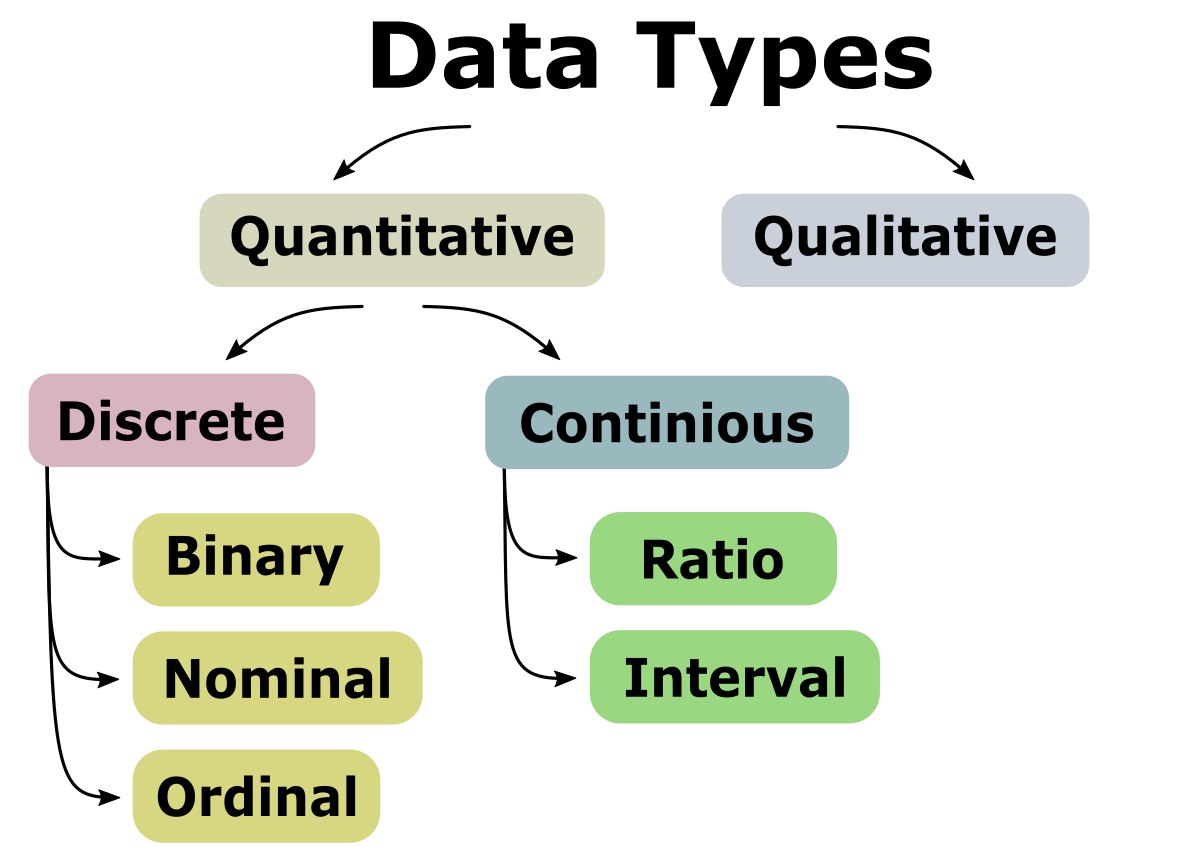
\includegraphics[scale=0.36]{assets/lectures_part_5-a3868f99.png}
\end{center}
\begin{itemize}
    \item \textbf{\color{javared} Кiлькiснi данi } використовують чисельнi значення для опису об’єкта, що нас цiкавить.
    \begin{itemize}
        \item \textbf{\color{javadocblue}Дискретнi данi} вiдповiдають вибiрцi з дискретного розподiлу г.с.
Дискретнi данi зазвичай є цiлими числами, хоча можуть задаватись i десятковими
дробими. Їх особливiстю є те, що вони мають ”пробiли” (”дiри”) у своїх можливих
значеннях.
\item
\textbf{\color{javadocblue}Неперервнi данi} вiдповiдають вибiрцi з неперервного розподiлу г.с.
Неперервнi данi приймають будь-якi значення з певного дiапазону i не мають
стрибкiв
    \end{itemize}
\item \textbf{\color{javared}Якiснi данi} використовують описовi вирази для вимiрювання або класифiкацiї об’єкта,
що нас цiкавить.
\end{itemize}
\newpage
\subsection{Первинна обробка інформації.}
\begin{itemize}
    \item \textbf{\color{javared}Варіаційним рядом} $x_{(1)} \leq x_{(2)} \leq \cdots \leq x_{(n)} $ називаються елементи вибiрки, якi
впорядкованi за зростанням. При цьому:
$$
x_{(1)} = \min\limits_{1 \leq k \leq n} x_k \qquad \quad x_{(n)} = \max\limits_{1 \leq k \leq n} x_k
$$
$x_k$ називається \textbf{\color{javadocblue}порядковою статистикою порядку k}.
\end{itemize}
Процес впорядкування вибiрки називається \textbf{\color{javadocblue}''ранжуванням''}.\par
\red{Розмах вибiрки} $R$ --- рiзниця мiж найбiльшим та найменшим елементами, тобто:
$$
R = x_{(n)} - x_{(1)}
$$
Нехай розподіл г.с. $F$ є дискретним. Тодi нехай $x_1^* , \dots , x_m^*$ – елементи вибiрки, впорядкованi
за зростанням, причому кожне значення вказується лише один раз, $n_k$ – число разiв появи $x_k^*$ в реалiзацiї вибiрки.  $n_k$ називається \blue{частотою} появи $x_k^*$.\par
Зауважимо, що $n_1 + \dots + n_m = n$.\par
Сума частот елементiв $ \displaystyle\sum\limits_{i = 1}^{ \textbf{k}}{x_i^*}$ називається \red{кумулятивною частотою} $n_k^*$:
$$
n_k^* = n_1 + ... + n_k
$$
Величина $\nu_k = \dfrac{n_k}{n}$ називається \red{вiдносною частотою}.
